\documentclass[a4paper,UTF8]{ctexart}

\usepackage{amssymb,amsmath}
\usepackage[top=1in,bottom=1in,left=1.5in,right=1.5in]{geometry}
\setlength{\columnsep}{0.5cm}
\usepackage[setpagesize=false, % page size defined by xetex
            unicode=false, % unicode breaks when used with xetexw
            xetex]{hyperref}
\usepackage[usenames,dvipsnames]{color}
\usepackage{listings}                     % 代码环境
\usepackage{xcolor}
\lstset{numbers = left,                   % 设置行号位置
        numberstyle = \tiny,          % 设置行号大小
        keywordstyle = \color{blue!70},                                         % 设置关键字颜色
        commentstyle = \color{red!50!green!50!blue!50},             % 设置注释颜色
        frame = single,               % 设置边框格式
        rulesepcolor = \color{red!20!green!20!blue!20},
        escapeinside = `',                  % 逃逸字符,用于显示中文
        xleftmargin = 1em, xrightmargin = 1em, aboveskip = 1em,     % 设置边框边距          
        tabsize = 4,                        % 设置tab空格数
        showspaces = false,                 % 不显示空格
        extendedchars = false,
        flexiblecolumns,              % 字列非等宽
        breaklines                          % 自动将长代码换行排版
        }
\usepackage{graphicx}                     % 插图  
\usepackage{subfigure}              % 实现图片并排
\usepackage{float}                  % 强制图片位置
\hypersetup{breaklinks=true,
            bookmarks=true,
            pdfauthor={徐孟莹 无35~~2013011161 ; 陈馨瑶 无35~~2013011166 ; 李思涵 无36~~2013011187},
            pdftitle={开放研究型实验},
            colorlinks=true,
            citecolor=blue,
            urlcolor=blue,
            linkcolor=magenta,
            pdfborder={0 0 0}}
\urlstyle{same}  % don't use monospace font for urls

\providecommand{\tightlist}{%
  \setlength{\itemsep}{0pt}\setlength{\parskip}{0pt}}
\setcounter{secnumdepth}{5}

\title{开放研究型实验}

\author{徐孟莹\\
无35~~2013011161\\ \and 陈馨瑶\\
无35~~2013011166\\ \and 李思涵\\
无36~~2013011187\\
\end{tabular}
\begin{tabular}{c}
\{xumy13,chenxinyao13,lisihan13\}@mails.tsinghua.edu.cn
}

\date{}

% Redefines (sub)paragraphs to behave more like sections
\ifx\paragraph\undefined\else
\let\oldparagraph\paragraph
\renewcommand{\paragraph}[1]{\oldparagraph{#1}\mbox{}}
\fi
\ifx\subparagraph\undefined\else
\let\oldsubparagraph\subparagraph
\renewcommand{\subparagraph}[1]{\oldsubparagraph{#1}\mbox{}}
\fi

\begin{document}
\maketitle

{
\hypersetup{linkcolor=black}
\setcounter{tocdepth}{3}
\tableofcontents
}

\section{背景}
% By 徐孟莹


\section{原理及方案设计}
% By 李思涵


\section{实验步骤}

\subsection{登陆}
% By 李思涵


\subsection{抓取最新微博}
% By 徐孟莹


\subsection{抓取话题关注者}
% By 徐孟莹


\subsection{抓取个人关注列表}
% By 陈馨瑶
抓取个人关注列表的函数接口如下:
\begin{lstlisting}[language = python]
def followings(self, uid):
\end{lstlisting}
其中,uid是需要抓取的用户的uid,函数的返回值是该用户关注的人的uid。

抓取过程如下:

利用GET请求访问以下网址
\begin{lstlisting}[language = python]
r = self.get('http://m.weibo.cn/page/json?containerid=100505%s_-_FOLLOWERS&page=%d' % (uid, i))
\end{lstlisting}
通过控制page的值就可以达到访问关注列表的不同页的目的。

解析所获得的数据结构,关注人的信息存储在$['cards'][0]['cards\_group']$下,进一步,可以从$['user']['id']$中得到关注人的uid。

进一步,为了应对经常性的抓取不成功和存在限制的情况,引入try结构,若三次抓取不成功则退出函数。


\subsection{抓取用户信息}
% By 李思涵


\subsection{用户信息统计}
% By 陈馨瑶
用户信息统计主要统计了话题关注者和话题参与者各自的年龄分布、性别分布和地理位置分布。除此以外,我还统计了抓下来的微博的转发数、评论数、点赞数分布和微博的发送时间分布(精确到小时),具体的步骤如下:

首先读取文件,关注者的信息存储在followers.pickle中,以用户的ID作为字典的键值。话题参与者的信息存储在data.pickle的$data['topic\_participants']$中,他们发送的微博的信息则存储在$data['topic\_posts']$中。在统计话题参与者和关注者的信息时,采用的数据结构如下:
\begin{lstlisting}[language = Python]
count = {
      'location': {},
      'age': {},
      'gender': {}
}
\end{lstlisting}

在统计话题微博的信息时,采用的数据结构如下:
\begin{lstlisting}[language = Python]
count = {
      'repost_num': {'0': 0, '1~5': 0, '5~10': 0, '10~15': 0, '15~20': 0, '20~50': 0, '50~100': 0, '>=100': 0},
      'comment_num': {'0': 0, '1~5': 0, '5~10': 0, '10~15': 0, '15~20': 0, '20~50': 0, '50~100': 0, '>=100': 0},
      'like_num': {'0': 0, '1~5': 0, '5~10': 0, '10~15': 0, '15~20': 0, '20~50': 0, '50~100': 0, '>=100': 0},
      'day': {},
      'hour': {}
}
\end{lstlisting}

在读取数据时,以用户信息统计为例,首先根据其数据结构得到每个人的地理位置、年龄和性别信息,以该信息作为键值,在count中判断该键是否存在。如果不存在,则新设置该键并将对应的值置为1,如果存在,则在原始值的基础上累加。在进行微博相关信息的统计时则采用了区间判断的方式,并对发送时间进行分割,提取出小时数。将最后统计得到的结果输入一个csv文件,便于用Excel进行作图。










\subsection{社交网络分析}
% By 徐孟莹


\section{结果}

\subsection{用户/微博分析}
% By 陈馨瑶

需要说明的是,我们所抓取的热门话题为“最好的我们”,这是一部青春校园爱情网剧。此外,在统计中出现的“-1”,指的是该用户并未设置这一信息或设置的该信息为空。

\subsubsection{话题关注者}

话题关注者的信息存储在followers.pickle中,编写程序对其进行分类和计数。其中,用户的地理位置信息只统计了省份的分布,作出的分布图如下:
\begin{figure}[H]
      \centering
      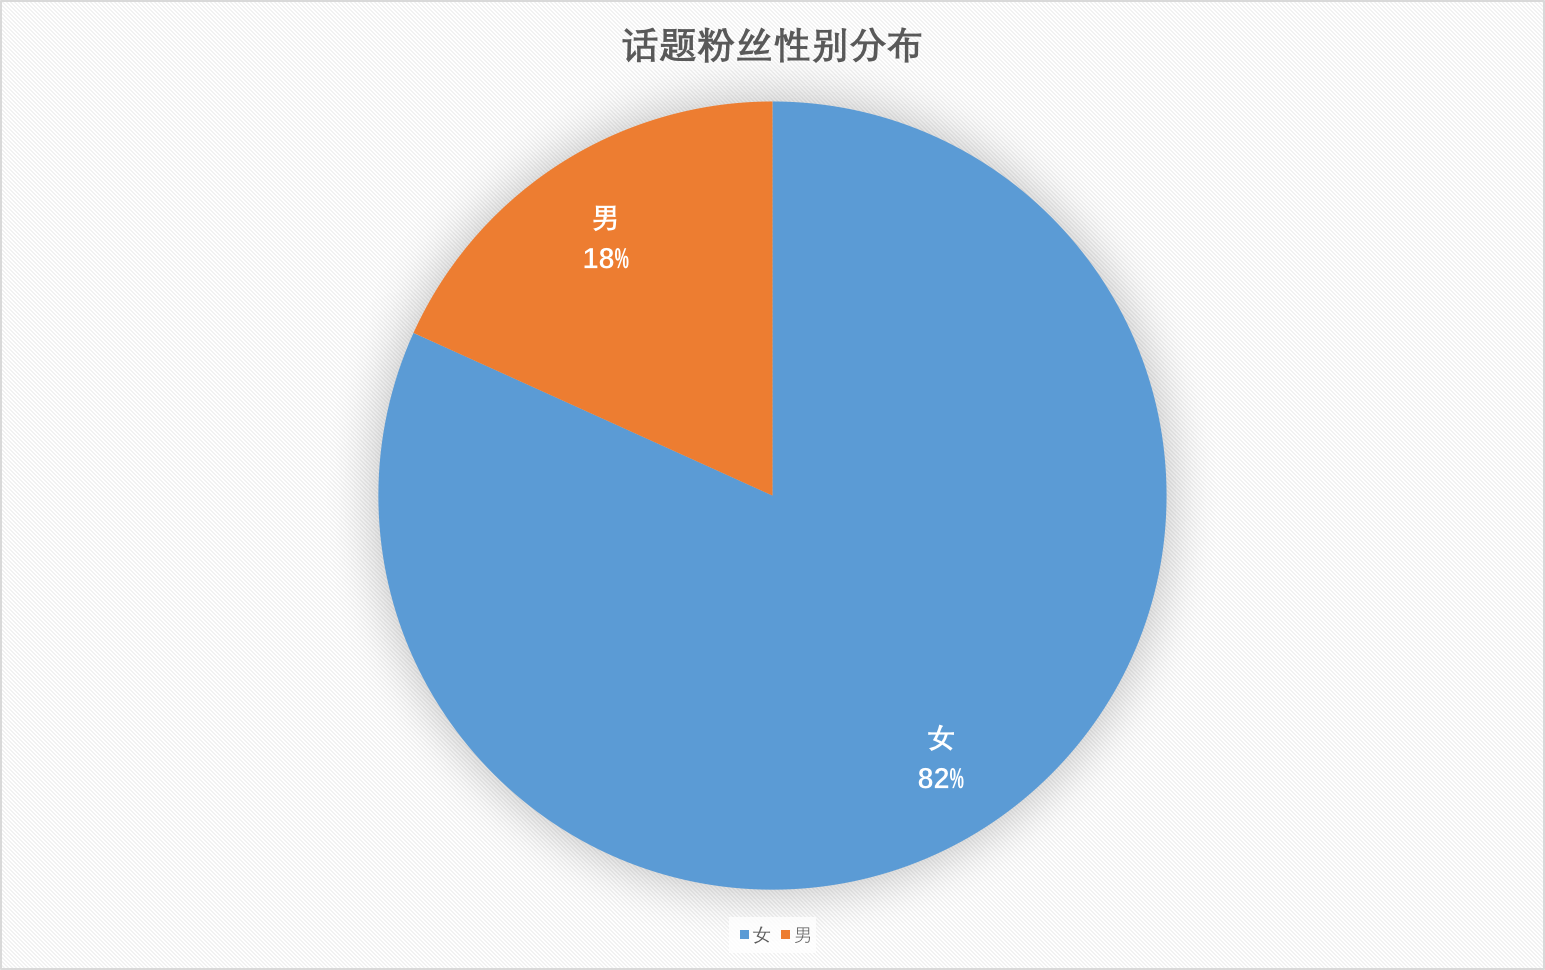
\includegraphics[width = \textwidth]{img/followers_gender.png}
      \caption{话题关注者性别分布}
\end{figure}

可以看到,该话题的关注者中,女性的比例要远远大于男性,这和这部剧的定位也是较为一致的。

\begin{figure}[H]
      \centering
      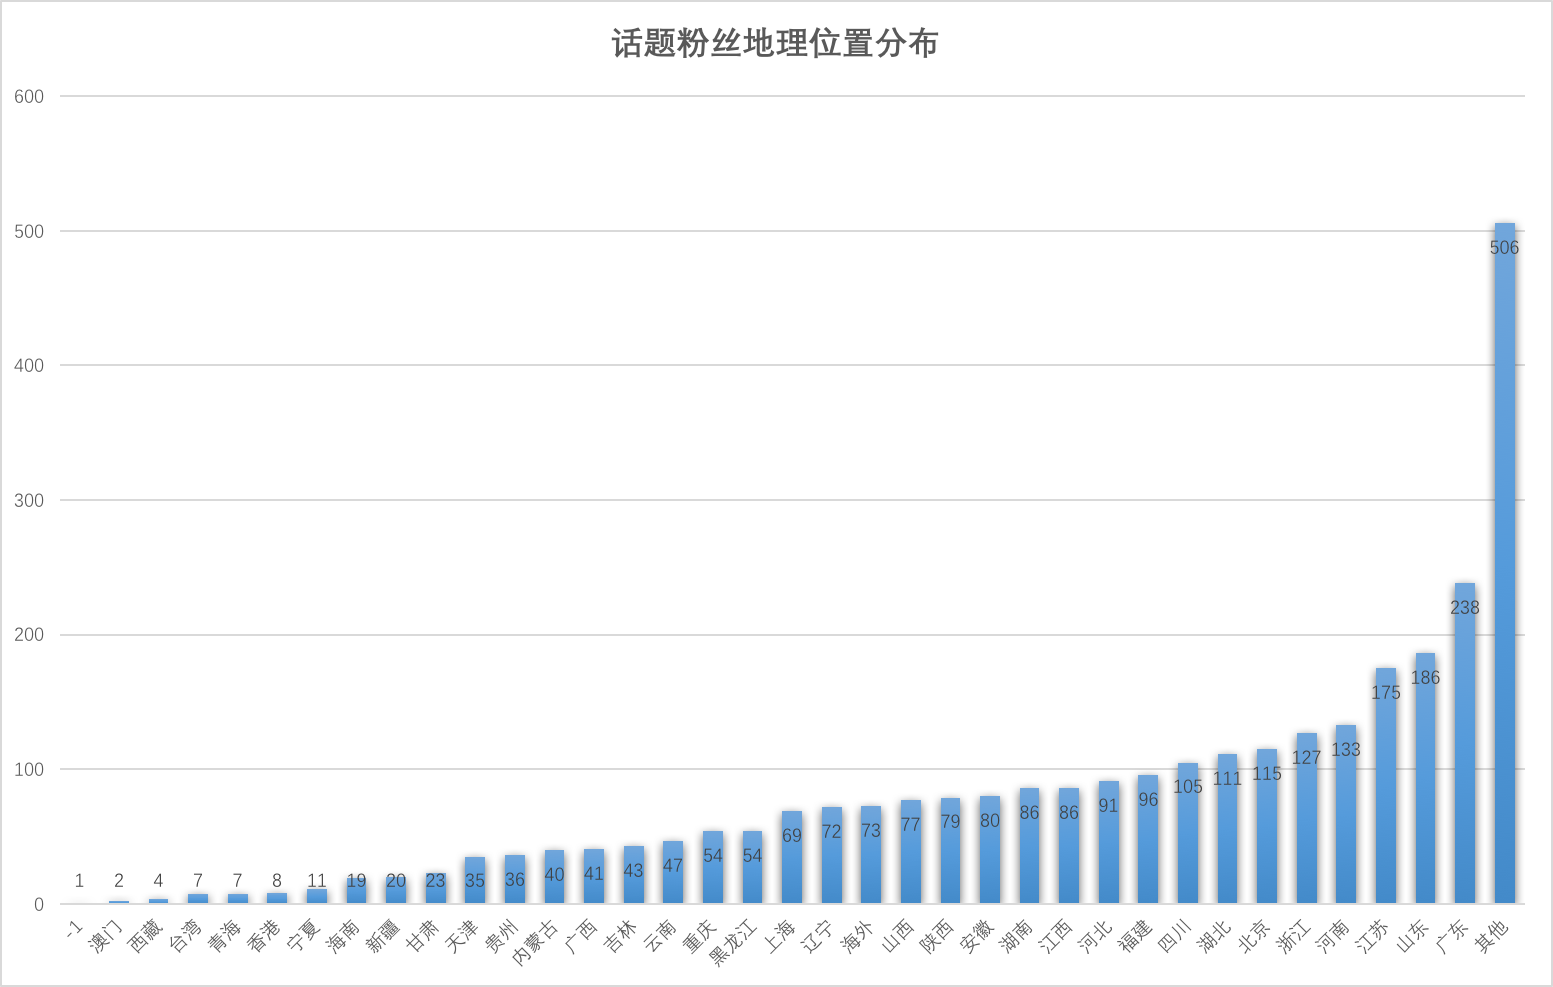
\includegraphics[width = \textwidth]{img/followers_location.png}
      \caption{话题关注者地理位置分布}
\end{figure}

在用户的地理位置分布中,占比最高的是“其他”,即这部分用户并未透露自己的地理位置信息,根据我对微博的了解,设置为其他的常常有如下几种情况:
\begin{itemize}
      \item 不愿意透露自己的个人信息
      \item 一些营销号性质的账户或僵尸粉
\end{itemize}
由此也不难解释为何“其他”会占如此大的比重。

在剩余的分布中,根据趋势,我认为各省市的人数分布和其经济状况以及人口数目呈正相关的关系。

\begin{figure}[H]
      \centering
      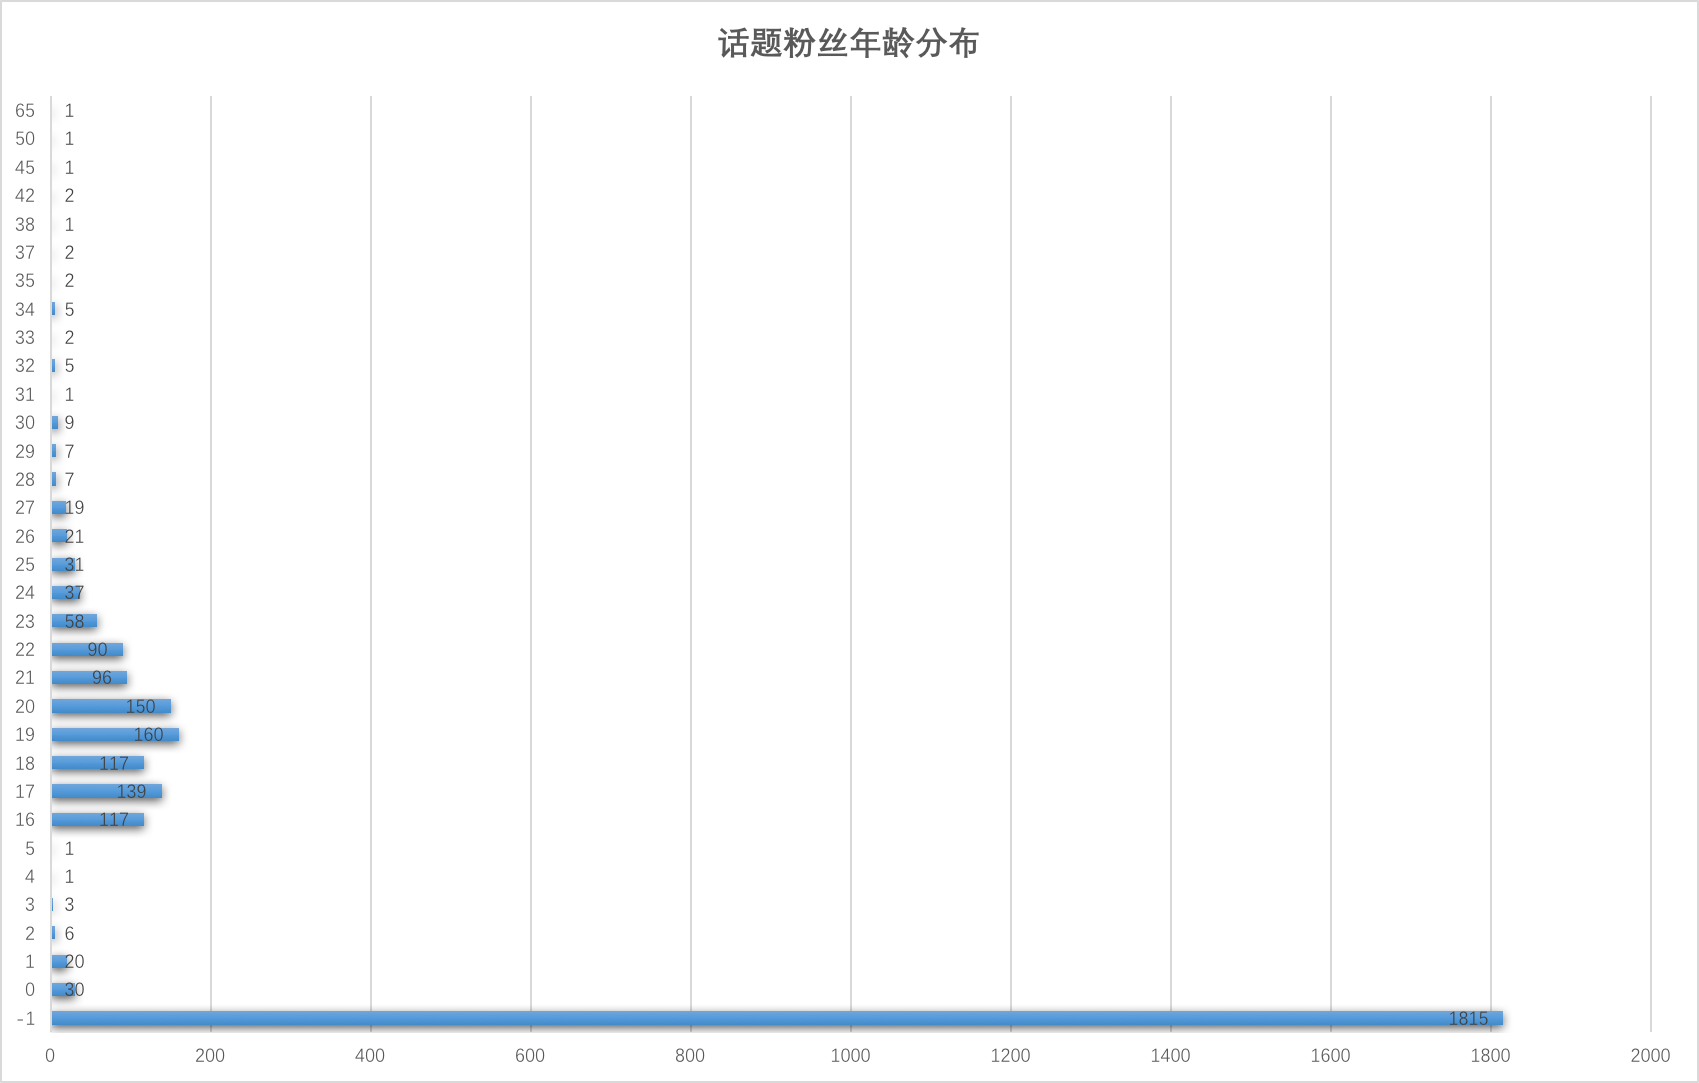
\includegraphics[width = \textwidth]{img/followers_age.png}
      \caption{话题关注者年龄分布}
\end{figure}

\subsubsection{话题讨论者}

\subsubsection{微博信息统计}

\subsection{社交网络分析}
% By 李思涵


\section{总结}
% By 陈馨瑶

\end{document}
